\chapter{Methodology}
\label{ch:method}

\begin{figure}[!ht]
	\centering
	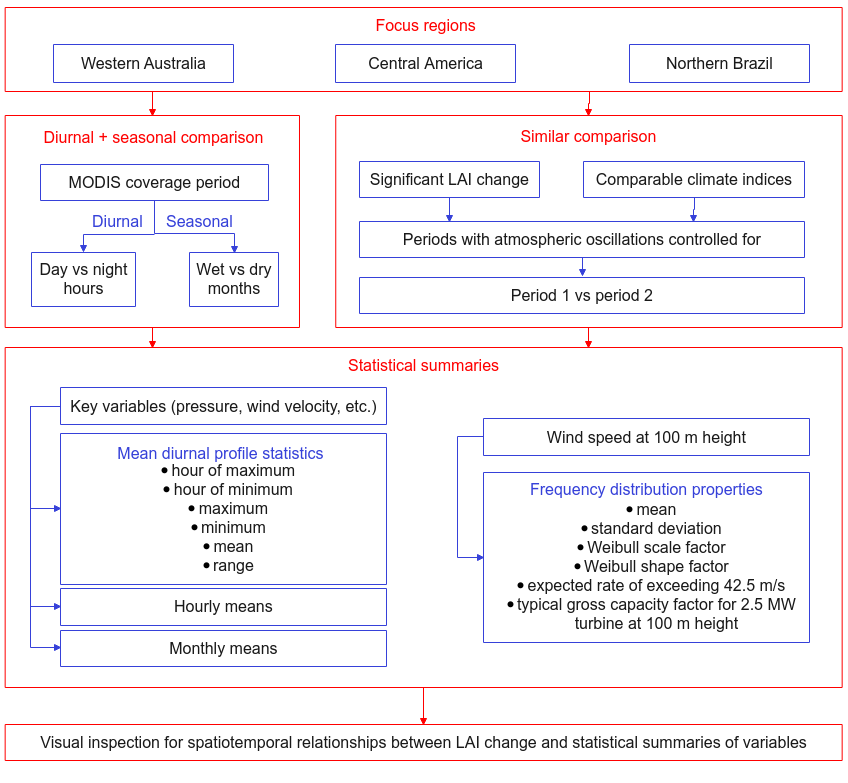
\includegraphics[width=0.9\textwidth]{method_flow}
	\caption[Methodology Flow Chart]{Flow chart summary for methodology.}
	\label{fig:method_flow}
\end{figure}

\section{Approach}

To identify how vegetation loss may affect (or has historically affected) surface winds, we produced a series of spatial plots using \ac{GLASS} data \citep{liang2021} and \ac{ERA5} data \citep{era5}. These plots sought to uncover any spatiotemporal correlations between vegetation loss and key atmospheric variables such as wind speed, wind direction and mean sea level pressure. The rationale behind this was that were there to be any concrete spatiotemporal correlations, it would suggest strongly that there is some underlying dynamic between the variables (since a concrete pattern manifesting through both space and time purely by chance is unlikely), which may then shed some insight into how atmospheric circulations may change in the future.

In doing this, we first identified three focus regions which were likely to yields results either due to historically extensive degrees of vegetation change or other unique circumstances such as having a sharp delineation between natural and agricultural land cover. For each of these regions, we produced two comparisons. The first comparison was between the dry and wet seasons (which can have significant differences in vegetation) for the period from Jan-2001 to Dec-2020\footnote{All period start and end dates in this report are inclusive unless otherwise stated.} (years in which available \ac{GLASS} data was most reliable due to an advancement of instruments), and will hereby be referred to as the "seasonal comparison". For the second comparison, we strategically selected two 5-year long historical periods with similar atmospheric conditions but extensive vegetation change, hereby referred to as the "similar comparison". Periods for the similar comparison were selected in such a fashion so as to control (to the extent possible) for other effects such as atmospheric oscillations which may also affect the key atmospheric variables of interest (mainly wind speeds, wind velocities and mean sea level pressure).

For each of these comparisons, we then created a series of spatial plots displaying summary statistics for the key atmospheric variables (see Section~\ref{sec:method_var}), as well as differences in these statistics between seasons or periods (other related variables which might affect the behaviour of the key variables were also studied).

Central to these summary statistics was a variable's \ac{MDP} over each period, produced using a group-wise average by hour of day for all the data values in that period. This was computed for each grid cell in the data, and was used to study how vegetation change might affect the diurnal variations in key variables. Because of the difficulty in visualising the temporal variability in spatial data, we created plots for the hour of maximum, hour of minimum, maximum, minimum, mean and range of these \ac{MDP} values. We also created spatial plots for the mean values over each hour of the day and month of the year, to analyse cotemporaneous diurnal and seasonal evolution of different variables respectively.

In addition to this, we created spatial plots for the wind speed distributional properties over each period (and the difference in these values between periods) for the wind speed at 100 m above surface such as its standard deviation, gross capacity factor for a typical wind turbine with 100 m hub height, empirical fits for the Weibull parameters, and the expected rate of exceeding 42.5 m/s (the typical speed which a turbine can withstand for 10 minutes).

Spatiotemporal correlations were then identified by visual inspection as this was deemed more appropriate than a rigid statistic metric, since the latter will have to be computed upon gridded data and hence may miss spatial correlations between variables which are present but manifest slightly offset from each other by a few grid cells (and it is a non-trivial task to systematically correct for all the different spatial variations by which two variables can be slightly offset from each other, if possible at all).

\section{Focus regions}

\subsection{Western Australia}

\begin{figure}[!ht]
	\centering
	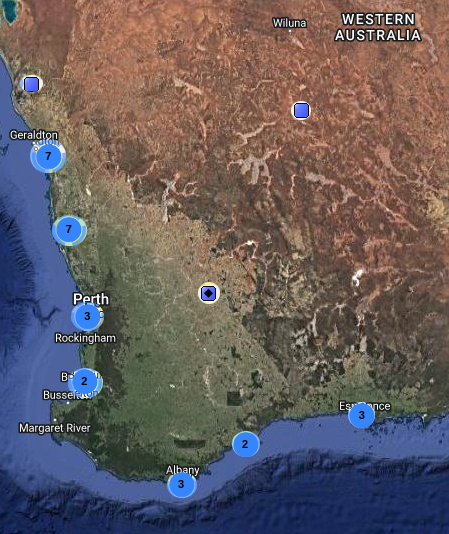
\includegraphics[width=0.9\textwidth]{maps_twp_wa}
	\caption[Western Australia Map]{Satellite image displaying Western Australia focus region from 114$^\circ$E to 124$^\circ$E longitude and 36$^\circ$S to 6$^\circ$S latitude \citep{maps_wa}. Markers indicating positions and number of wind farms have been edited on using data from \citep{twp_wa}. The State Boundary Fence of Western Australia sharply delineates agricultural vegetation on the west from native vegetation on the east.}
	\label{fig:maps_twp_wa}
\end{figure}

We selected the south-west part of \ac{WA} (from 114$^\circ$E to 124$^\circ$E longitude and 36$^\circ$S to 6$^\circ$S latitude; see Figure~\ref{fig:maps_twp_wa}) for investigation because previous studies \citep{lyons1993, lyons1996, lyons2002, xinmei1995, ray2003, esau2002} have suggested significantly different atmospheric conditions on each side of the \ac{SBFWA}, which itself sharply delineates native vegetation (on the eastern side) from agricultural land (on the western side).

Land surface characteristics on the agricultural side exhibit pronounced seasonal fluctuations due to the annual growing and harvest of wheat, after which the ground is left bare before the next growing season. Furthermore, land usage on each side of the fence has remained the same over recent decades. This focus region was selected mostly for these unique characteristics which are conducive towards eliciting insights into the general principles tying land cover with atmospheric circulation, but may also have some direct implications for wind farms in the area.

As illustrated in Figure~\ref{fig:maps_twp_wa}, there are several wind farms within this region, mostly along the coast. Vegetation change on an annual to decadal scale has been concentrated along the south-western coastal forests (see Section~\ref{sec:results_wa}), while effects on a seasonal scale will be most pronounced along the fence. Wind farms around these regions are the ones most likely to see a change in wind resource due to continued forest loss and future agricultural expansion respectively.

\subsection{Central America}

\begin{figure}[!ht]
	\centering
	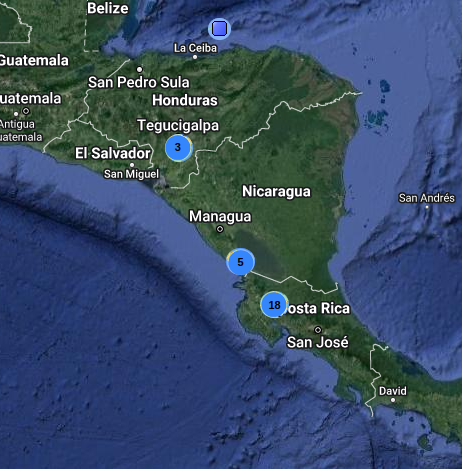
\includegraphics[width=0.9\textwidth]{maps_twp_ca}
	\caption[Central America Map]{Satellite image displaying Central America focus region from 91$^\circ$W to 81$^\circ$W longitude and 17$^\circ$S to 7$^\circ$S latitude \citep{maps_ca}. Markers indicating positions and number of wind farms have been edited on using data from \citep{twp_hd, twp_nc, twp_cr}.}
	\label{fig:maps_twp_ca}
\end{figure}

We selected the part of \ac{CA} which runs (North to South) from El Salvador and Honduras to Nicaragua to Costa Rica (91$^\circ$W to 81$^\circ$W longitude and 17$^\circ$S to 7$^\circ$S latitude; see Figure~\ref{fig:maps_twp_ca}) because there existed spatially opposing trends in vegetation change. These countries had historically comparable rates of deforestation, but Costa Rica shifted towards reforestation due to policy changes in the 1990s whereas deforestation has continued in Honduras and Nicaragua. The western coastlines for El Salvador, Nicaragua and Costa Rica (where agriculture is concentrated) also have comparable cardinal orientations.

Being located near the equator, annual temperature variation at these locations are relatively minor. This is useful because it provides a comparison where one of the main variables affecting wind flow is relatively controlled for. Furthermore, the entire focus region is on the order of 1000 km, so synoptic weather features (which have a characteristic scale of this order) are less likely to produce contrasting effects over the different subregions\footnote{This comment also applies for the \ac{WA} case.}.

Wind farms are concentrated on agricultural land along the western coast where there are plans for continued development. But as in the case of \ac{WA}, the value of this focus region isn't necessarily in its direct implications for existing wind farms in the area, but in that it may yield some insights into the principles between land cover change and surface winds, which may then have broader implications for wind energy generation in general.

\subsection{Northern Brazil}

\begin{figure}[!ht]
	\centering
	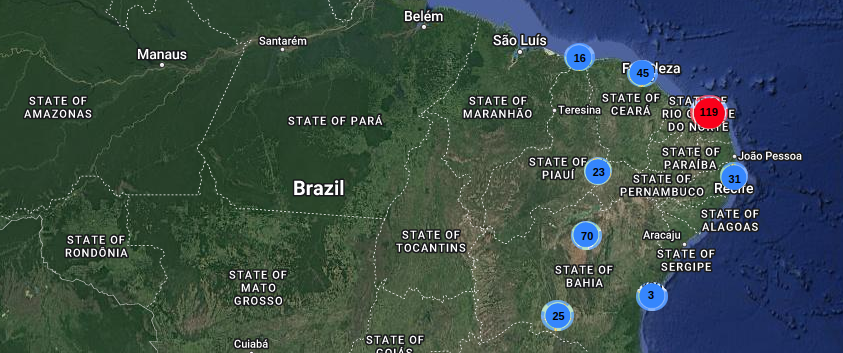
\includegraphics[width=0.9\textwidth]{maps_twp_sa}
	\caption[Northern Brazil Map]{Satellite image displaying Northern Brazil focus region from 65$^\circ$W to 30$^\circ$W longitude and 15$^\circ$S to 0$^\circ$S latitude \citep{maps_sa}. Markers indicating positions and number of wind farms have been edited on using data from \citep{twp_br}.}
	\label{fig:maps_twp_sa}
\end{figure}

We selected the North to Northeast regions of Brazil (65$^\circ$W to 30$^\circ$W longitude and 15$^\circ$S to 0$^\circ$S latitude; see Figure~\ref{fig:maps_twp_sa}) because there has been extensive deforestation over this area and it was believed that effects resulting from \ac{LCC} here were likely to be especially pronounced.

Several studies have identified large-scale changes in precipitation and moisture convergence patterns, which indirectly implicate surface wind changes. Effects here are likely to have immediate implications for energy generation due to the number of wind farms in this region (both existing and in the development pipeline\footnote{Up to 60 GW of offshore wind near the northeastern coast is in the early planning stage \citep{offshore_map}.}).

\section{Study periods}

\subsection{General}

\subsubsection{Wet and dry months}

Based on historical precipitation climatology, we have selected the months representing the wet and dry seasons for each region as being:
\begin{itemize}
	\item \ac{WA}: June, July, August (JJA) and December, January, February (DJF) respectively
	\item \ac{CA}: May to October (5-6-7-8-9-10) and November to April (1-2-3-4-11-12) respectively
	\item \ac{NB}: January to June (1-2-3-4-5-6) and July to December (7-8-9-10-11-12)
\end{itemize}

\subsubsection{Daytime and nighttime hours}

The local timezones for \ac{WA}, \ac{CA} and \ac{NB} are UTC+8, UTC-6 and UTC-3 respectively\footnote{The focus region for \ac{NB} spans across 35 degrees of longitude, so it actually covers multiple local timezones and over more than 2 hours of local solar timezones (15 degrees per hour). We have selected UTC-3 here because this is close to the local solar timezone for the midpoint of this region.}. Where comparisons between daytime and nighttime hours have been made, the average values for hours from 8 am to 3 pm local time\footnote{Unless otherwise stated, all times in this report are expressed in local time, and hour endpoints are inclusive.} (8-9-10-11-12-13-14-15) have been selected as representative of daytime, while the average values for hours from 8 pm to 3 am local time (0-1-2-3-20-21-22-23) have been selected as representative of nighttime.

\subsection{Seasonal comparison}

For all focus regions, the seasonal comparison is performed over the period from Jan-2001 to Dec-2020 (inclusive). The GLASS products derived from \ac{MODIS}, the more advanced instrument, begin around Mar-2000, with the \ac{LAI} dataset ending Dec-2021 while the \ac{FAPAR} dataset ends Dec-2020 (at the time of writing). As averages starting from Mar-2000 and ending Dec-2020 would have skewed weightings for the months of January and February, we elected to use Jan-2001 as the period start instead.

\subsection{Similar comparison}

To control for differences arising from atmospheric oscillations, and to select periods for which there was sufficient vegetation change for meaningful results to appear, we selected a set of study periods for each region based on the following criteria (in order of priority):
\begin{enumerate}
	\item 5-year rolling averages for relevant climate indices were similar or at a similar phase in the oscillation
	\item Change in \ac{LAI} between the periods was extensive or had opposite trends in different subregions
	\item Monthly values for relevant climate indices over each period displayed a similar time evolution pattern
	\item Periods covered a similar amount of time spent in La Nina / El Nino events (where relevant) and Negative / Positive \ac{IOD} events (where relevant)
\end{enumerate}

Period lengths of 5 years were selected since this somewhat averages out the effect of shorter-term atmospheric fluctuations. To assist in the selection of periods, we created 5-year rolling average line plots for the climate indices corresponding to each region's relevant (i.e. climate-driving) atmospheric oscillations (see Section~\ref{ssec:indices}). We also created yearly spatial plots for the 5-year rolling average of the annual difference in \ac{MLAI} (see Section~\ref{ssec:mlai_diff}).

\subsubsection{Climate indices}
\label{ssec:indices}

5-year rolling average line plots were produced for the following climate indices using monthly data obtained from \ac{NOAA} \citep{ind_source}:
\begin{itemize}
	\item \ac{AMOI}, for the \ac{AMO}
	\item \ac{PDOI}, for the \ac{PDO}
	\item \ac{ONI}, for the \ac{ENSO}
	\item \ac{DMI}, for the \ac{IOD}
	\item \ac{AAOI}, for the \ac{AAO} / \ac{SAM}
	\item \ac{AOI}, for the \ac{AO} / \ac{NAM}\footnote{The \ac{AO} is actually quite distant from all the focus regions and was not a major factor in selection of periods but was included in the analysis for completeness.}
	\item \ac{NAOI}, for the \ac{NAO}
	\item \ac{EPOI}, for the \ac{EPO} / \ac{NPO}
\end{itemize}

Overlayed upon the \ac{ONI} graphs were windows indicating when La Nina and El Nino events have occurred in the past, as defined by the \ac{JMA}.\footnote{Note that different meteorological agencies define these events differently. \ac{JMA} definitions were used here because it was the only data down to a monthly resolution which was easily obtainable.} And overlayed upon the \ac{DMI} graphs were windows indicating when Negative \ac{IOD} and Positive \ac{IOD} events have occurred in the past, as defined by \ac{JMA}.

\subsubsection{Annual difference in mean leaf area index}
\label{ssec:mlai_diff}

For each calendar year with completed data in the \ac{GLASS} dataset, an annual mean value was computed for the \ac{LAI} at each grid point. The annual difference in \ac{MLAI} for each year was then defined as the \ac{MLAI} for that year minus the mean of the previous year. A 5-year rolling average centred upon each year was then produced by averaging the four annual differences calculated across the five annual means. For example, the 5-year rolling average for the year 2002 would be the average of $MLAI(2004)-MLAI(2003)$, $MLAI(2003)-MLAI(2002)$, $MLAI(2002)-MLAI(2001)$ and $MLAI(2001)-MLAI(2000)$, where the \ac{MLAI} over a given year is expressed as $MLAI(year)$.

This averages out the shorter term fluctuations which may be due to rainfall anomalies around a mean trend, or other factors such as changes in cropping. Although interesting in their own right, these are only indirectly related to \ac{LCC} (the subject of this report) and so are not pursued.

As the time difference between similar periods in terms of climate indices often exceeds 5 years, these plots were used only as a visual indicator to aid the selection process (to determine whether periods with sufficiently similar climate indices would also have extensive enough vegetation change to be worth studying). For final confirmation, separate comparison plots for the \ac{MLAI} over each of the selected 5-year periods were produced.

\section{Variables selected for analysis}
\label{sec:method_var}

Variables which were analysed are presented in Table~\ref{tab:vars_analysis}. The \ac{LSE} and \ac{SSGO} were static variables derived from the \ac{ERA5} dataset, used to identify whether orographically-induced circulations would be a confounding factor. \ac{MLAI} was the primary metric used to assess the extent of vegetation change, with \ac{MFAPAR} a secondary metric to corroborate results. 

We then selected out for analysis the \ac{ERA5} variables which were most relevant to our research goals. \ac{MSLP}, \ac{WS100} (the relevant height for wind generation) and \ac{WV100} were natural inclusions given we are analysing the wind resource. But also included were variables targeted towards understanding the processes behind these circulations, such as on surface energy balance, atmospheric energy budget and possible effects of atmospheric condensation.

There was an emphasis on variables related to water vapour transport, not only because of the potential for \ac{CIAD}, but also because this provides relatively high-fidelity data to corroborate the direction of tropospheric winds with that on the surface. Modelled outputs for water vapour transport are forced using satellite observations, and itself constitutes indirect measurement of tropospheric winds. But vegetation-surface wind interactions in ERA5 are modelled by extrapolating downwards from a fixed blending height and using grids with a characteristic roughness. As a result, the accumulated effects of sub-grid heterogeneity upon the trajectory of winds may not be accounted for, and in either case the surface winds are at least an extra step removed from direct measurement\footnote{Observations assimilated into the model for ERA5 do not include wind velocity inputs from weather stations because ERA5 is averaged over 0.25$^\circ$ grids which makes it incompatible with WMO conventions whereby 10 m winds are measured in open terrain. Instead, 100 m winds are extrapolated downwards from higher model levels under idealised assumptions, and the data assimilated for these higher model levels in turn derives from a mix of atmospheric soundings, aircraft and satellite irradiance data (part of which relies back on water vapour observations).}

We also derived a variable called \ac{NAC}, which was meant to approximate the instantaneous balance between cloud formation and cloud evaporation at each hour of the day (see Appendix~\ref{sec:nac_derive} for derivation):
\begin{eqnarray}
	\label{eq:nac}
	NAC \ [kg m^{-2} s^{-1}] = NSE \ [kg m^{-2} s^{-1}] - VIDMF \ [kg m^{-2} s^{-1}] \\ 
	- \frac{d}{dt}(TCWV \ [kg m^{-2}]) \nonumber
\end{eqnarray}
where \acs{NSE} is the net evaporation at the surface (i.e.\ not including atmosphere), \acs{VIDMF} is the vertical integral of divergence of moisture flux, and \acs{TCWV} is the total column water vapour (see descriptions in Table~\ref{tab:vars_analysis}).

This is an accounting equation arising from the fact that \ac{TCWV} can only change either due to net evaporation or condensation (on the surface and also in the atmosphere), or movement of water vapour from a neighbouring column (it is also theoretically possible for chemical reactions and sublimation/deposition to add or remove water vapour but this is assumed negligible). This equation is usually expressed in the atmospheric water vapour budget literature \citep{norris2020, yan2020} as
\begin{eqnarray}
	\frac{d}{dt}(TCWV) = E - P - VIDMF
\end{eqnarray}
where E is surface evaporation and P is precipitation. But this equation is only valid for larger spatial and temporal scales. 

At larger temporal scales, surface evaporation at the surface typically exceeds surface condensation, so \ac{NSE} will be positive and is expressed as E (but note that this is using a more abstract notion of “surface evaporation” which absorbs the effect of intermittent surface condensation within the study period). To avoid confusion, we retain the use of the term “NSE” which makes explicit that surface condensation is absorbed within this variable. 

Also, this literature equation is only valid if P = NAC. All atmospheric condensation eventually falls as precipitation so this equation is valid on larger spatial and temporal scales. But on smaller scales, there may be several hours of delay between condensation and precipitation, and winds may blow the condensed water droplets across several hundred km before precipitating. Since we are studying hourly diurnal profiles and using 30 km grids, we opt for \ac{NAC} rather than P in this equation.

By similar reasoning, the use of \ac{TCCLW} may give misleading results since prevailing winds may low cloud liquid water far from their point of formation. Thus, \ac{NAC} is meant to provide a more accurate depiction of where cloud formation is occurring.

Also included in Table~\ref{tab:vars_analysis} are descriptions for wind speed distribution properties derived from \ac{ERA5} data (see Section~\ref{ssec:method_wsd}).

\begin{landscape}
%	\pagestyle{empty} %% only if you want to remove silly headers on the side	
	\begingroup
	\renewcommand\arraystretch{1.33} % only applicable to this table because of group

		\begin{longtable}{P{2cm}P{3cm}P{15cm}}
			\caption[Study Variables]{Variables which were analysed. Abbreviations for these variables as used in this report are provided, along with descriptions of each variable.} 
			\label{tab:vars_analysis} 
			\\ 
			\toprule 
			\multicolumn{1}{P{2cm}}{\textbf{Abbreviation}}
			& \multicolumn{1}{P{3cm}}{\textbf{Variable}}
			& \multicolumn{1}{P{15cm}}{\textbf{Description}}\\	
			\midrule
			\endfirsthead
			\midrule
			\multicolumn{1}{P{2cm}}{\textbf{Abbreviation}}
			& \multicolumn{1}{P{3cm}}{\textbf{Variable}}
			& \multicolumn{1}{P{15cm}}{\textbf{Description}}\\	
			\midrule	
			\endhead
			\midrule	
			\multicolumn{3}{l@{}}{(continued\ldots)}\\
			\endfoot
			\endlastfoot
			LSE & Land Surface Elevation & Units in $m$. Elevation of the land surface above seas level. Obtained by converting from ERA5 geopotential data using the MetPy python library \citep{metpy}. \\
			SSGO & Slope of Sub-Gridscale Orography & Dimensionless. Represents slopes of orographic features such as mountains and hills which are present down to a scale of 1 km. Flat surfaces have value 0 while vertical cliffs have value 1. \\ \midrule
			MLAI & Mean Leaf Area Index & Dimensionless. The leaf area index for a grid cell is the total leaf area divided by ground area of that cell. MLAI is the mean of this over the study period. This was the main metric used in assessing vegetation cover and vegetation cover change.  \\
			MFAPAR & Mean Fraction of Photosynthetically Absorbed Radiation & Dimensionless. The fraction of photosynthetically absorbed radiation for a grid cell is the fraction of radiation between 400-700 nm wavelength absorbed within that cell. MFAPAR is the mean of this over the study period. This was a supplementary metric used in assessing vegetation cover and vegetation cover change. \\ \midrule
			BLH & Boundary Layer Height & Units in $m$. Height of the depth of air for which surface effects are significant. This was used to assess level of convective mixing and likelihood fo cloud formation. \\
			CAPE & Convective Available Potential Energy & Units in $J kg^{-1}$. Work which would be performed on an air parcel if it rose through the atmosphere. This was used to indicate atmospheric stability. The more positive the more air will rise, the more negative the more air will sink. \\
			CBH & Cloud Base Height & Units in $m$. Height for base of lowest cloud. This was used to assess how height of cloud formation may affect atmospheric circulations. \\
			FA & Forecast Albedo & Dimensionless. Fraction of short-wave radiation reflected from surface. This was used to assess how reflectivity of different land cover affects the surface energy balance. \\
			MSLP & Mean Sea Level Pressure & Units in $Pa$. Pressure of atmosphere adjusted to sea level. This is one of the main variables affecting wind. High values typically coincide with calm conditions while low values coincide with windy. This was also used to identify synoptic features. \\
			NAC & Net Atmospheric Condensation & Units in $kg m^{-2} s^{-1}$. Condensation minus evaporation in atmosphere (does not include surface). Positive values indicate more cloud formation than cloud evaporation. Calculated using ERA5 data for TCWV, NSE and VIDMF (see Appendix~\ref{sec:nac_derive}). This is one of the major factors affecting the partitioning of the atmospheric energy budget. \\
			NSE & Net Surface Evaporation & Units in $kg m^{-2} s^{-1}$. Evaporation minus condensation at surface (does not include atmosphere). For vegetation, positive values indicate a greater amount of evapotranspiration than dew formation. Instantaneous values are approximated by averaging consecutive ERA5 accumulation values.\footnote{ERA5 parameters come in instantaneous and accumulation values. Instantaneous values are calculated for that point in time at each hour whereas accumulation values represent a sum compiled over the course of the previous hour window. NSE, SLHF and SSHF are accumulation values whereas the remainder are instantaneous. Averages for these variables were computed to approximate "instantaneous" values in order to allow an apples to apples comparison.} \\
			SLHF & Surface Latent Heat Flux & Units in $W m^{-2}$. Rate at which energy at the surface is being used for evapotranspiration. Instantaneous values are approximated by averaging consecutive ERA5 accumulation values (see NSE footnote). \\
			SSHF & Surface Sensible Heat Flux & Units in $W m^{-2}$. Rate at which energy at the surface is being used to induce convection and warming of the air mass above it. Instantaneous values are approximated by averaging consecutive ERA5 accumulation values (see NSE footnote). \\
			T2 & Temperature at 2 m Above Surface & Units in $K$. This is one of the major factors affecting the partitioning of the atmospheric energy budget. \\
			TCC & Total Cloud Cover & Dimensionless. Fraction of grid cell covered by cloud. \\
			TCCLW & Total Column Cloud Liquid Water & Units in $kg m^{-2}$. Total cloud liquid content averaged over grid cell. Does not include rain water droplets. \\
			TCWV & Total Column Water Vapour & Units in $kg m^{-2}$. Total amount of water vapour averaged over grid cell. Often referred to as precipitable water (PW). \\
			U10 & Zonal Component of 10 m Wind Velocity & Units in $m s^{-1}$. East-West component of wind velocity at 10 m above surface. Positive values indicate that wind has a westerly component (blowing \textit{to} the east). \\
			U100 & Zonal Component of 10 m Wind Velocity & Units in $m s^{-1}$. East-West component of wind velocity at 100 m above surface. Positive values indicate that wind has a westerly component (blowing \textit{to} the east). \\
			V10 & Meridional Component of 10 m Wind Velocity & Units in $m s^{-1}$. North-South component of wind velocity at 10 m above surface. Positive values indicate that wind has a southerly component (blowing \textit{to} the north). \\
			V100 & Meridional Component of 100 m Wind Velocity & Units in $m s^{-1}$. North-South component of wind velocity at 100 m above surface. Positive values indicate that wind has a southerly component (blowing \textit{to} the north). \\
			VIDMF & Vertical Integral of Divergence of Moisture Flux & Units in $kg m^{-2} s^{-1}$. The average rate at which water vapour in a grid cell is leaving to neighbouring grid cells.\footnote{Note that ERA5 has a similarly named parameter called "vertically integrated moisture divergence" (VIMD) which is an accumulation rather than instantaneous parameter, but with the crucial difference that "moisture" in this variable refers to the total of water vapour, cloud liquid and cloud ice. The ERA5 documentation for VIDMF also refers to "moisture" and it is not apparent that this actually uses a different definition where it only includes water vapour, but this was indeed confirmed to be the case via correspondence with ECMWF specialist support.} Positive values indicate water vapour is diverging (leaving grid cell) while negative values indicate water vapour is converging (entering grid cell). \\
			VIEC & Vertical Integral of Energy Conversion & Units in $W m^{-2}$. Rate at which energy is being converted from internal plus potential energy into kinetic energy.\footnote{By ERA5 definitions, internal energy refers to the microscopic energy of the air molecules excluding latent energy (this is treated as a separate part of the atmospheric energy budget) which may be different to definitions used in chemistry. Potential energy here refers to macroscopic gravitational potential energy (as opposed to internal air pressure within the grid cell, as this is implicitly accounted for within internal energy). Kinetic energy refers to kinetic energy from the \textit{horizontal} motion of air masses.} Negative values indicate kinetic energy conversion into internal plus potential energy. \\
			VIKE & Vertical Integral of Kinetic Energy & Units in $J m^{-2}$. Total kinetic energy from the \textit{horizontal} motion of air masses through the grid cell, averaged over the grid cell. This was used to study how land cover change affects partitioning in the atmospheric energy budget. \\
			VIPILE & Vertical Integral of Potential, Internal and Latent Energy & Units in $J m^{-2}$. Total of gravitational potential energy, internal energy and latent energy (see footnote for VIEC). This constitutes the total atmospheric energy budget minus kinetic energy. This was used to study how land cover change affects partitioning in the atmospheric energy budget. \\
			WS10 & Wind Speed at 10 m Above Surface & Units in $m s^{-1}$. Scalar quantity for wind speed at 10 m above surface. \\
			WS100 & Wind Speed at 100 m Above Surface & Units in $m s^{-1}$. Scalar quantity for wind speed at 100 m above surface. This is the quantity most directly relevant for wind energy generation. \\
			WV10 & Wind Velocity at 10 m Above Surface & Units in $m s^{-1}$. Vector quantity for wind velocity at 10 m above surface. \\
			WV100 & Wind Velocity at 100 m Above Surface & Units in $m s^{-1}$. Vector quantity for wind velocity at 100 m above surface. This quantity is also directly relevant for wind energy generation and furthermore highlights how wind direction changes. \\ \midrule
			d\{VAR\} & Hourly Change in \{VAR\} & Units vary. Change in the value for each of the above ERA5 or ERA5-derived values, as compared with its value in the previous hour. This was used to study how the rate of change of a variable was correlated with land cover change. \\ \midrule
			C10 & Weibull Scale Parameter for 10 m Wind Speed & Units in $m s^{-1}$. Scale parameter for the Weibull distribution fit to the wind speed at 10 m above surface. The empirical Weibull fit was obtained using the equations of \citep{justus1977}. \\
			C100 & Weibull Scale Parameter for 100 m Wind Speed & Units in $m s^{-1}$. Scale parameter for the Weibull distribution fit to the wind speed at 100 m above surface. The empirical Weibull fit was obtained using the equations of \citep{justus1977}. \\
			EROE100 & Expected Rate of 100 m Wind Speed Exceeding 42.5 m/s & Dimensionless. The \textit{expected} rate for wind speed at 100 m exceeding 42.5 m/s, which in practice is the typical wind speed which wind turbines can last 10 mins in before failure \citep{chen2015, chen2016, ge_web}. This is the \textit{expected} rate calculated from the tail of the Weibull distribution fit rather than the actual observed rate of exceedance. \\
			K10 & Weibull Shape Parameter for 10 m Wind Speed & Dimensionless. Shape parameter for the Weibull distribution fit to the wind speed at 10 m above surface. The empirical Weibull fit was obtained using the equations of \citep{justus1977}. \\
			K100 & Weibull Shape Parameter for 100 m Wind Speed & Dimensionless. Shape parameter for the Weibull distribution fit to the wind speed at 100 m above surface. The empirical Weibull fit was obtained using the equations of \citep{justus1977}. \\
			$mean$(WS10) & Mean of 10 m Wind Speed & Units in $m s^{-1}$. Mean of wind speed at 10 m above surface. This is roughly equivalent to the mean of the mean diurnal profile for WS10 (see Section~\ref{ssec:method_mdp}). \\
			$mean$(WS100) & Mean of 100 m Wind Speed & Units in $m s^{-1}$. Mean of wind speed at 10 m above surface. This is roughly equivalent to the mean of the mean diurnal profile for WS100 (see Section~\ref{ssec:method_mdp}). \\
			$std$(WS10) & Standard Deviation of 10 m Wind Speed & Units in $m s^{-1}$. Standard deviation of wind speed at 10 m above surface. This is used with K10 to analyse how the variability in wind speed changes along with land cover. \\
			$std$(WS100) & Standard Deviation of 100 m Wind Speed & Units in $m s^{-1}$. Standard deviation of wind speed at 10 m above surface. This is used with K100 to analyse how the variability in wind speed changes along with land cover. \\
			TGCF100 & Gross Capacity Factor for Typical Turbine at 100 m Above Surface & Dimensionless. Gross capacity factor which a typical 2.5 MW turbine with 100 m hub height would have had over the study period. This was computed by first averaging the power curves for similar 2.5 MW turbines from Vestas, Goldwind and GE Energy, then computing the energy generation for each hour in the study period using ERA5 data for the wind speed at 100 m above surface (see Section~\ref{ssec:method_wsd}). \\ \bottomrule
		\end{longtable}

	\endgroup
\end{landscape}

\section{Statistical summaries}
\label{sec:method_stats}

\begin{figure}[!ht]
	\centering
	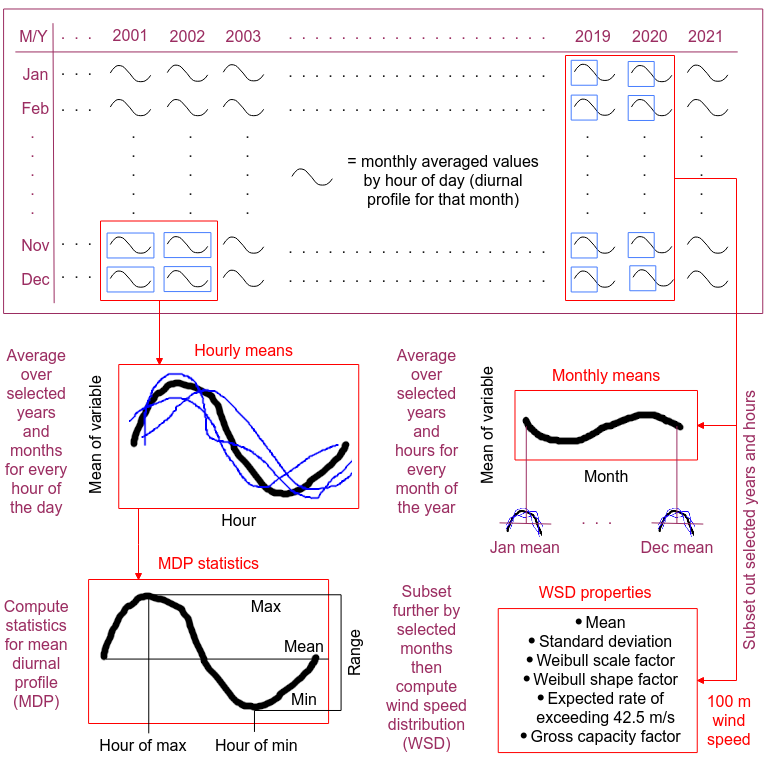
\includegraphics[width=0.9\textwidth]{stats_flow}
	\caption[Statistics Flow Chart]{Flow chart illustrating how the statistical summaries for each variable were computed.}
	\label{fig:stats_flow}
\end{figure}

\subsection{Mean diurnal profile statistics}
\label{ssec:method_mdp}

The "mean diurnal profile" (\ac{MDP}) for a variable was defined by computing groupwise means for values by hour of day\footnote{These averages were produced mostly by computing the mean of monthly averaged by hour of day data, which is roughly equivalent to the mean of all hourly data values. Vector variables were computed using hourly data values rather than monthly averaged by hour of day. Reasons for these choices are discussed in Appendix~\ref{sec:commutativity}.}. That is, the mean over all data values occurring on the first hour of the day were computed, then the same was done for the second and all subsequent hours up until the 24th hour, and together these constitute the \ac{MDP}. The \ac{MDP} can be computed upon a month subset of the total data available over a period, so \ac{MDP}s using values only from the wet or dry season can be obtained. 

The hour of maximum, hour of minimum, maximum, minimum, mean and range for the \ac{MDP} at each grid cell was then computed for visualisation\footnote{Note here that for variables which can take on both positive and negative values, maximum refers to the most positive \ac{MDP} value and minimum refers to the most negative \ac{MDP} value.}. Because, hour of maximum, hour of minimum, maximum, minimum and range for a vector is not well defined, we choose to apply generalised definitions for these statistics here so that: \ac{MDP} hour of maximum and minimum refers to when the \ac{MDP} magnitude of vector $\vec{v}$ is at a maximum and minimum respectively, \ac{MDP} maximum and minimum refers to the \ac{MDP} vector quantity of $\vec{v}$ at the hour of maximum and minimum, and \ac{MDP} range refers to largest magnitude of all possible subtractions (corresponding to all possible hourly combinations) between the 24 \ac{MDP} $\vec{v}$ values. Formally:
\begin{eqnarray}
	hour_{max}(\vec{v}) = i \mbox{ where } |\vec{v}_i| = max( \{|\vec{v}_k| : k \in \mathbb{Z} \cap [1,24] \}) \\
	hour_{min}(\vec{v}) = j \mbox{ where } |\vec{v}_j| = min( \{|\vec{v}_k| : k \in \mathbb{Z} \cap [1,24] \}) \\
	max(\vec{v}) = \vec{v}_i \mbox{ where } |\vec{v}_i| = max( \{|\vec{v}_k| : k \in \mathbb{Z} \cap [1,24] \}) \\
	min(\vec{v}) = \vec{v}_j \mbox{ where } |\vec{v}_j| = min( \{|\vec{v}_k| : k \in \mathbb{Z} \cap [1,24] \}) \\
	mean(\vec{v}) = \frac{1}{24} \sum_{k=1}^{24} \vec{v}_k \\
	range(\vec{v}) = max(\{|\vec{v}_k - \vec{v}_l| : k,l \in \mathbb{Z} \cap [1,24] \})
\end{eqnarray}

\subsection{Hourly means}

Hourly mean values are equivalent to the actual hourly values which constitute the \ac{MDP} (as opposed to the \ac{MDP} statistics).

\subsection{Monthly means}

Monthly mean values are similar to hourly means except that it is computed separately for every month of the year (rather than a collection of months corresponding to wet or dry season), and instead can be computed over a subset of hours for comparison between day and night hours.

\subsection{100 m wind speed distribution}
\label{ssec:method_wsd}

For the wind speed distribution, the sample mean and standard deviation was first obtained over the selected months and hours subset. An empirical Weibull fit was then performed in accordance with the methodology outlined by \citep{justus1977}:
\begin{eqnarray}
	k = \left( \frac{\sigma}{\bar{V}} \right)^{-1.086} \\ 
	c = \frac{\bar{V}}{\Gamma (1 + 1/k)}
\end{eqnarray}
where $k$ is the Weibull shape parameter, $c$ is the Weibull scale parameter, $\sigma$ is the standard deviation of wind speed, $\bar{V}$ is the mean of wind speed, and $\Gamma (z) = \int_0^\infty t^{z-1} e^{-t} dt$ is the gamma function.

\ac{EROE100} was then calculated using the tail from the empirical Weibull fit (as opposed to rate of exceedance directly calculated from the hourly data points) since the underlying probability distribution better captures risks which by chance may not have manifested in the data points. 42.5 m/s was chosen as this is the typical wind speed which wind turbines can last 10 mins in before failure \citep{chen2015, chen2016, ge_web}.

Experimental results by \citet{lee2012} and a review of methods by \citet{palutikof1999} suggest that the use of a Gumbel distribution for wind gust data would have been more accurate for assessing extreme wind speeds, but this analysis was not pursued since the ERA5 dataset does not contain a field for wind gusts at 100 m, and because interpretation of Gumbel parameters are less intuitive.

As opposed to EROE100, \ac{TGCF100} was directly calculated from the hourly data points. This was deemed valid because tail wind speeds have an insignificant effect on \ac{TGCF100} as all wind speeds above the cutoff represent zero power anyway. \ac{TGCF100} was calculated by first averaging the power curves of three turbines by common manufacturers to obtain a typical power curve, then using this to calculate the average power generated over the period as a fraction of the nameplate power rating.\footnote{Note that this is mathematically equivalent to computing the gross capacity factor for each of the three turbines then finding the average (see Appendix~\ref{sec:commutativity}).} The Vestas V100/2600, Goldwind GW100/2500 and GE Energy 2.5-100 were chosen for this calculation since these were turbines at 100 m hub height with comparable rotor diameter (100 m), power rating (2500 kW), and cut-in and cut-off wind speeds.\footnote{The Vestas power curve was scaled by a factor of 25/26 to make it comparable with the other turbines.} Data for these turbine power curves were obtained from \citet{twp_ge, twp_gw, twp_vt}.

\section{Main datasets}

\subsection{ERA5 reanalysis data}

The \ac{ERA5} dataset is provided by \ac{ECMWF} and is widely used in atmospheric studies. We required reanalysis data to visualise changes over an entire region (as opposed to in-situ measurements which are usually sparse). Of the available reanalysis datasets, ERA5 was chosen for its superior spatial (0.25$^\circ$) and temporal (hourly) resolution, closest agreement with observed wind speeds, and relatively accurate capture of interannual variability \citep{ramon2019, torralba2017}.

The superior resolution was particularly important since this project sought to investigate diurnal variations (so an hourly time resolution was desirable), and the methodology was designed to interrogate the interfaces between different types of land cover (coarser spatial resolutions may have averaged out interesting effects).

\subsection{GLASS satellite-derived data}

The \ac{GLASS} product suite includes spatially complete modelled datasets for \ac{LAI} and \ac{FAPAR} with temporal resolution of 8 days (constrained by satellite overpasses) and spatial resolutions down to 250 m. This dataset is widely used for analysing vegetation cover and land surface effects \citep{liang2021}, and was selected because it was found to be the most consistent with Google Earth historical satellite imagery. The datasets with spatial resolution of 0.05$^\circ$ were selected as this provided sufficient detail to distinguish land cover types at sharp interfaces without consuming too much computer storage and memory.

Other datasets such as the \ac{ERA5} \ac{LAI} variables, unprocessed {AVHRR}/{MODIS} satellite observations, \ac{ECMWF} \ac{LAI} V3 and \ac{NOAA} \ac{CDR} \ac{NDVI} V5 were considered, but these were found to often have missing values, data processing artefacts, discrepancy against Google Earth imagery, or other significant data deficiencies (not shown).

\section{Software}

All data manipulations were performed using Python 3.9.12. Statistical summaries were computed primarily using the \verb+xarray+ \citep{xarray} and \verb+dask+ \citep{dask} libraries, while visualisations relied on the \verb+matplotlib+ \citep{matplotlib} and \verb+cartopy+ \citep{cartopy} libraries.

A series of purpose-designed Python programs were created in the course of this project. These programs include a \verb+data_download.py+ script to automatically download all raw data inputs used in this project, a \verb+calc_funcs.py+ script which handles all the data processing, and a \verb+plot_funcs.py+ script which handles all the visualisations. 

All programs created in the course of this project are freely available, and all results were designed to be reproducible from scratch (see Appendix~\ref{app:code}). With trivial edits, these programs can take an arbitrary variable from the ERA5 dataset, then compute and visualise the statistical summaries outlined in Section~\ref{sec:method_stats}. These programs have broader applicability beyond this project as it can be used to study diurnal and seasonal variations in general, as well as how these variations differ between periods.

Due to the memory requirements necessary to process the large datasets, this research includes computations using the computational cluster Katana supported by Research Technology Services at \ac{UNSW} Sydney.